\chapter{Numerical Optimization and Training of Neural Networks}

\section{Introduction: the Perceptron}

The first model that introduced the idea of a neural network was the perceptron. 
The perceptron is a simple model that takes a set of inputs and produces an output. 
The model is based on the idea of a neuron in the brain, which receives signals from 
other neurons and produces an output signal.\\

The perceptron is a linear model that takes a set of binary inputs 
$x = (x_1, x_2, \ldots, x_n)$ and produces an output $y$ in the following way:

\begin{equation}
    y = \begin{cases}
        1 & \text{if } w_1 x_1 + w_2 x_2 + \ldots + w_n x_n + b > 0\\
        0 & \text{otherwise}
    \end{cases}
\end{equation}

where $w = (w_1, w_2, \ldots, w_n)$ are the weights of the model and $b$ is the bias.
Note that this can be represented as a vector product:

\begin{equation}
    y = \begin{cases}
        1 & \text{if } w \cdot x + b > 0\\
        0 & \text{otherwise}
    \end{cases}
\end{equation}

The perceptron is a simple model that can be used to classify data into two classes.
The model is trained by adjusting the weights and bias to minimize the error on the 
training data.\\

Note that the perceptron is a linear model, which means that it can only learn linearly
separable functions. This means that the model can only learn functions that can be
separated by a hyperplane. If the data is not linearly separable, the perceptron will 
not be able to learn the function.\\

This problem is illustrated by the XOR function, which is not linearly separable.

\subsection{The XOR problem}

The XOR logical function is a simple function that takes two binary inputs and 
produces an output, which is 1 if the inputs are different and 0 if the inputs 
are the same. The XOR function is defined as follows:

\begin{table}[H]
    \centering
    \begin{tabular}{|c|c|c|}
        \hline
        $x_1$ & $x_2$ & $y$\\
        \hline
        0 & 0 & 0\\
        0 & 1 & 1\\
        1 & 0 & 1\\
        1 & 1 & 0\\
        \hline
    \end{tabular}
    \caption{XOR function}
\end{table}

Note that the XOR function is not linearly separable, i.e., it is not possible to
separate the data points with a hyperplane. For instance, the following plot shows
the XOR function in the input space:

\begin{figure}[H]
    \centering
    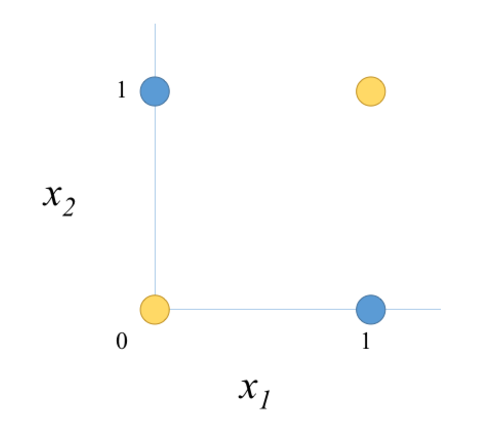
\includegraphics[width=0.5\textwidth]{figures/xor_plot.png}
    \caption{XOR function in the input space}
    \label{fig:xor_plot}
\end{figure}

As we can see, the data points are not linearly separable, which means that 
the perceptron alone cannot learn the XOR function. This is a limitation of
the perceptron model. However, let us take a look at how we can overcome this
limitation by using a more complex model: the multi-layer perceptron.

\subsection{NAND gate}

The NAND gate is a simple logical function that takes two binary inputs and
produces an output, which is 0 if both inputs are 1 and 1 otherwise. The NAND
gate is defined as follows:

\begin{table}[H]
    \centering
    \begin{tabular}{|c|c|c|}
        \hline
        $x_1$ & $x_2$ & $y$\\
        \hline
        0 & 0 & 1\\
        0 & 1 & 1\\
        1 & 0 & 1\\
        1 & 1 & 0\\
        \hline
    \end{tabular}
    \caption{NAND gate}
\end{table}

The NAND gate is an example of a function that is linearly separable, i.e., it can
be separated by a hyperplane. This means that the perceptron can learn the NAND
gate function. Notice that the NAND gate is an universal gate, which means that
it can be used to implement any logical function. This is an important property
of the NAND gate, as it allows us to build more complex functions using simple
building blocks.\\

Because the NAND gate can represent any logical function by combining multiple
gates, and the perceptron can learn the NAND gate, we can use the perceptron to
learn any logical function, just by combining multiple perceptrons. This is the
raw idea behind the multi-layer perceptron.

\subsection{The problem of the step function}

Notice that the perceptron uses a step function to produce the output. It takes 
the value 1 if the input is greater than 0 and 0 otherwise. This has some problems,
as it implies that possible small changes in the input and weights can lead to a
discontinuous change in the output, i.e., big jumps in the output. This can make
the optimization process difficult.\\

To overcome this problem, we can use a different activation functions, such as the
sigmoid function, which is a smooth function that takes values between 0 and 1.
The idea of using a continuous activation function, combined with multiple layers
of perceptrons, is the basis of the multi-layer perceptron.


\section{The Multi-Layer Perceptron}

The multi-layer perceptron (MLP) is a neural network model that consists of multiple
layers of perceptrons. On the output layer, we use a different activation function
than the step function, such as the sigmoid function. This allows the model to learn
more complex functions, as it can approximate any continuous function.\\

We can represent the MLP model using a graph, where each node represents a perceptron
and each edge represents a weight. The graph is organized in layers, where each layer
is connected to the next layer. The input layer represents the input data, the output
layer represents the output of the model, and the hidden layers represent the intermediate
layers of the model.\\

\begin{figure}[H]
    \centering
    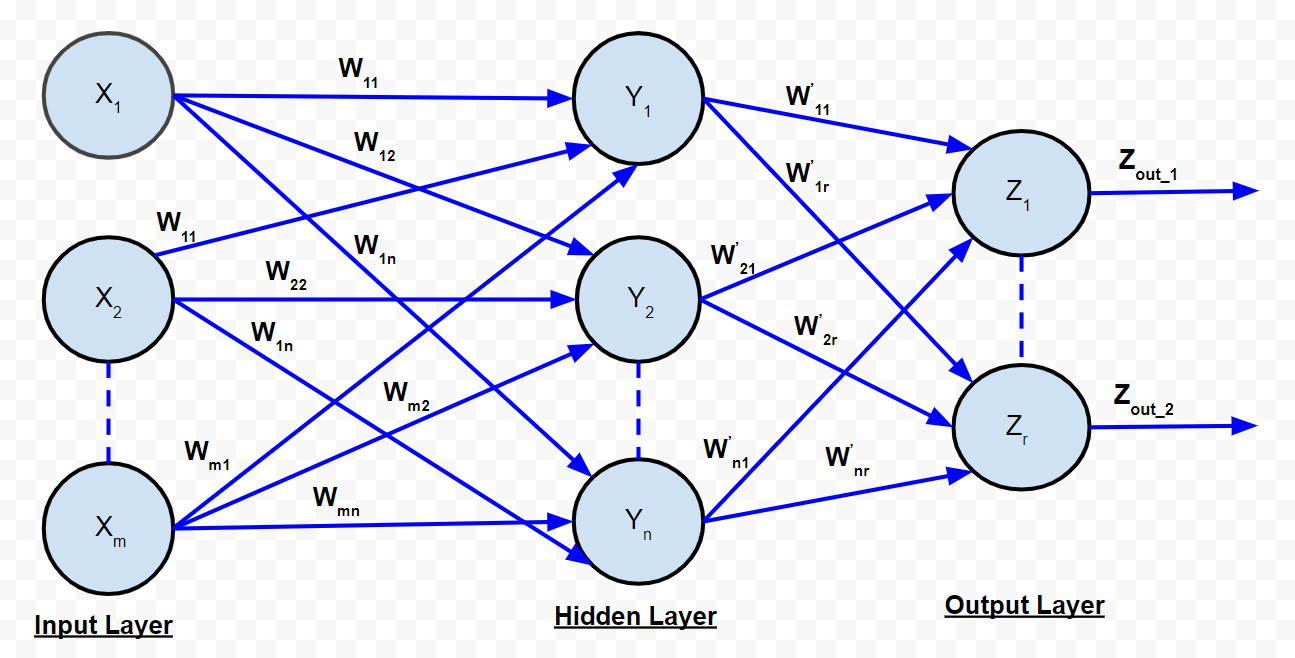
\includegraphics[width=0.7\textwidth]{figures/MLP.jpg}
    \caption{Graph representation of the MLP model}
    \label{fig:mlp_graph}
\end{figure}

For a neuron $j$ in layer $\ell$, we have the following:

\begin{equation}
    z_j^\ell = \sum_{k} w_{jk}^\ell a_k^{\ell-1} + b_j^\ell
\end{equation}

where $z_j^\ell$ is the weighted sum of the inputs of neuron $j$ in layer $\ell$,
$w_{jk}^\ell$ is the weight of the connection between neuron $k$ in layer $\ell-1$
and neuron $j$ in layer $\ell$, $a_k^{\ell-1}$ is the output after activation
of neuron $k$ in layer $\ell-1$, and $b_j^\ell$ is the bias of neuron $j$ in 
layer $\ell$.\\

Notice that in each output layer, we apply an activation function to the weighted sum
of the inputs. This activation function is a non-linear function that allows the model
to learn complex functions. This is represented by:

\begin{equation}
    a_j^\ell = \sigma(z_j^\ell)
\end{equation}

where $\sigma$ is the activation function. In general, we can represent the weights
as a matrix $W^\ell$ and the biases as a vector $b^\ell$. This allows us to write
the equation that represents the output of a particular layer as follows:

\begin{equation}
    a^\ell = \sigma(W^\ell a^{\ell-1} + b^\ell)
\end{equation}
    
where $a^\ell$ is the output of layer $\ell$, $a^{\ell-1}$ is the output of layer
$\ell-1$, and $\sigma$ is the activation function. This equation represents the
forward pass of the model, i.e., the process of computing the output of the model
given an input.\\

Now, on the output layer, we need a function that can represent the distance between
the output of the model and the true output. This function is called the loss function,
and it measures the error of the model. The main goal of training a neural network is
to minimize the loss function.

\section{Training a Neural Network}

To train a neural network, we need to define a loss function that measures the error
of the model. This function takes the
output of the model and the true output and produces a value that represents how
well the model is performing. In general, a loss function $J$ should have the 
following properties:

\begin{enumerate}
    \item $J$ can be written as an average of the loss over the training data.
    $$J = \frac{1}{N} \sum_{i=1}^{N} J_s$$
    where $N$ is the number of samples in the training data and $J_s$ is the loss
    for sample $s$.

    \item $J$ is a function only of the output of the model and the true output.
\end{enumerate}

Now, to train the model, we need to minimize the loss function. This is done by
adjusting the weights and biases of the model to reduce the error. This process
is called optimization. There are many optimization algorithms that can be used
to train a neural network, but in general, all of them follow the same idea:
compute the gradient of the loss function with respect to the weights and biases
and update the weights and biases in the opposite direction of the gradient.
This is called gradient descent.\\

Therefore, our aim is to compute the derivative of the loss function with respect
to the weights and biases of the model, i.e., we need to compute:

\begin{equation}
    \frac{\partial J}{\partial w^\ell_{jk}}, \frac{\partial J}{\partial b^\ell_j} \quad \forall \ell, j, k
\end{equation}

where $w^\ell_{jk}$ is the weight of the connection between neuron $k$ in layer $\ell-1$
and neuron $j$ in layer $\ell$, and $b^\ell_j$ is the bias of neuron $j$ in layer $\ell$.\\

For this, let us define the vector of errors (or sensitivities) $\delta^\ell$ for 
layer $\ell$ as follows:

\begin{equation}
    \delta^\ell_j = \frac{\partial J}{\partial z^\ell_j} \quad \forall j
\end{equation}

where $z^\ell_j$ is the weighted sum of the inputs of neuron $j$ in layer $\ell$.
The vector of errors $\delta^\ell$ represents how much the error changes with respect
to the weighted sum of the inputs of neuron $j$ in layer $\ell$.\\

Now, we will deduce 4 funcamental equations that will allow us to compute the
gradient of the loss function with respect to the weights and biases of the model.
These equations are called the backpropagation equations, and they are the key
to training a neural network.\\

\subsection{Backpropagation equations}

\begin{enumerate}
    \item Compute the error of the output layer $\delta^L$:
    
    $$\delta^L_j = \frac{\partial J}{\partial z^L_j} = \sum_{k} \frac{\partial J}{\partial a^L_k} \cdot \frac{\partial a^L_k}{\partial z^L_j} $$
    
    Because $a^L_k$ only depends on $z^L_k$ if $k = j$, we have:

    $$\delta^L_j = \frac{\partial J}{\partial a^L_j} \cdot \frac{\partial a^L_j}{\partial z^L_j}$$
    
    Notice that:
    $$\frac{\partial a^L_j}{\partial z^L_j} = \sigma'(z^L_j)$$ 
     
    where $\sigma'$ is the derivative of the activation function. Then, we have:

    $$\delta^L_j = \frac{\partial J}{\partial a^L_j} \cdot \sigma'(z^L_j)$$

    Notice that the value of $z^L_j$ has already been computed in the forward pass.
    Rewriting the equation in vector form, we have:

    \begin{equation}
        \delta^L = \nabla_{a^L} J \odot \sigma'(z^L)
    \end{equation}

    where $\nabla_a J$ is the gradient of the loss function with respect to the output
    of the model and $\odot$ is the element-wise product.

    \item Compute the error of the hidden layers $\delta^\ell$ with respect to $\delta^{\ell+1}$:
    
    $$\delta^\ell_j = \frac{\partial J}{\partial z^\ell_j} = \sum_{k} \frac{\partial J}{\partial z^{\ell+1}_k} \cdot \frac{\partial z^{\ell+1}_k}{\partial z^\ell_j}$$

    Notice that: 
    
    $$\frac{\partial J}{\partial z^{\ell+1}_k} = \delta^{\ell+1}_k$$

    Then, we have:

    $$\delta^\ell_j = \sum_{k} \delta^{\ell+1}_k \cdot \frac{\partial z^{\ell+1}_k}{\partial z^\ell_j}$$

    Now, we need to compute the derivative of $z^{\ell+1}_k$ with respect to $z^\ell_j$.
    Notice that:

    $$z^{\ell+1}_k = \sum_{m} w^{\ell+1}_{km} a^\ell_m + b^{\ell+1}_k  = \sum_{m} w^{\ell+1}_{km} \sigma(z^\ell_m) + b^{\ell+1}_k$$

    Then, we have:

    $$\frac{\partial z^{\ell+1}_k}{\partial z^\ell_j} = w^{\ell+1}_{kj} \cdot \sigma'(z^\ell_j)$$

    Finally, we have:

    $$\delta^\ell_j = \sum_{k} \delta^{\ell+1}_k \cdot w^{\ell+1}_{kj} \cdot \sigma'(z^\ell_j)$$

    Rewriting the equation in vector form, we have:

    \begin{equation}
        \delta^\ell = ((W^{\ell+1})^T \delta^{\ell+1}) \odot \sigma'(z^\ell)
    \end{equation}

    \item Compute the gradient of the loss function with respect to $b^\ell$:
    
    $$\frac{\partial J}{\partial b^\ell_j} = \frac{\partial J}{\partial z^\ell_j} \cdot \frac{\partial z^\ell_j}{\partial b^\ell_j}$$

    Notice that:

    $$z_j^\ell = \sum_{k} w_{jk}^\ell a_k^{\ell-1} + b_j^\ell$$

    Then, we have:

    $$\frac{\partial z^\ell_j}{\partial b^\ell_j} = 1$$

    Finally, we have:

    $$\frac{\partial J}{\partial b^\ell_j} = \delta^\ell_j$$

    Rewriting the equation in vector form, we have:

    \begin{equation}
        \nabla_{b^\ell} J = \delta^\ell
    \end{equation}

    \item Compute the gradient of the loss function with respect to $W^\ell$:
    
    $$\frac{\partial J}{\partial w^\ell_{jk}} = \frac{\partial J}{\partial z^\ell_j} \cdot \frac{\partial z^\ell_j}{\partial w^\ell_{jk}}$$

    Notice that:

    $$z_j^\ell = \sum_{k} w_{jk}^\ell a_k^{\ell-1} + b_j^\ell$$

    Then, we have:

    $$\frac{\partial z^\ell_j}{\partial w^\ell_{jk}} = a_k^{\ell-1}$$

    Finally, we have:

    $$\frac{\partial J}{\partial w^\ell_{jk}} = \delta^\ell_j \cdot a_k^{\ell-1}$$

    Rewriting the equation in matrix form, we have:

    \begin{equation}
        \nabla_{W^\ell} J = \delta^\ell (a^{\ell-1})^T
    \end{equation}

\end{enumerate}

These are the backpropagation equations, which allow us to compute the gradient of the
loss function with respect to the weights and biases of the model. This is the key to
training a neural network. By computing the gradient of the loss function and updating
the weights and biases in the opposite direction of the gradient, we can minimize the
error of the model and learn complex functions.\\

Summarizing the equations:

\begin{enumerate}
    \item Compute the error of the output layer:
    $$\delta^L = \nabla_{a^L} J \odot \sigma'(z^L)$$

    \item Compute the error of the hidden layers:
    $$\delta^\ell = ((W^{\ell+1})^T \delta^{\ell+1}) \odot \sigma'(z^\ell)$$

    \item Compute the gradient of the loss function with respect to $b^\ell$:
    $$\nabla_{b^\ell} J = \delta^\ell$$

    \item Compute the gradient of the loss function with respect to $W^\ell$:
    $$\nabla_{W^\ell} J = \delta^\ell (a^{\ell-1})^T$$
\end{enumerate}

Then, the backpropagation algorithm can be summarized as follows:

\begin{enumerate}
    \item $x$ is the input to the model. Compute $a^1$
    \item For each layer $\ell$ from $2$ to $L$:
    \begin{enumerate}
        \item Compute $z^\ell = W^\ell a^{\ell-1} + b^\ell$
        \item Compute $a^\ell = \sigma(z^\ell)$
    \end{enumerate}
    \item Compute the loss function $J$
    \item Compute the error of the output layer $\delta^L$
    \item For each layer $\ell$ from $L-1$ to $1$:
    \begin{enumerate}
        \item Compute the error of the hidden layers $\delta^\ell$
        \item Compute the gradient of the loss function with respect to $b^\ell$
        \item Compute the gradient of the loss function with respect to $W^\ell$
        \item Update the weights and biases:
        \begin{itemize}
            \item $W^\ell = W^\ell - \alpha \nabla_{W^\ell} J$
            \item $b^\ell = b^\ell - \alpha \nabla_{b^\ell} J$
        \end{itemize}

        where $\alpha$ is the learning rate.
    \end{enumerate}
\end{enumerate}

\section{Activation functions}

The activation function of a neuron is a non-linear function that takes the weighted
sum of the inputs of the neuron and produces an output. The activation function is
a key component of a neural network, as it allows the model to learn complex functions.
There are many activation functions that can be used in a neural network, but some
of the most common are:

\begin{enumerate}
    \item Sigmoid function:
    \begin{equation}
        \sigma(z) = \frac{1}{1 + e^{-z}}
    \end{equation}

    The sigmoid function takes values between 0 and 1, which makes it useful for
    binary classification problems. However, the sigmoid function has some problems,
    such as the vanishing gradient problem, which can make training difficult.

    \item Hyperbolic tangent function:
    \begin{equation}
        \tanh(z) = \frac{e^z - e^{-z}}{e^z + e^{-z}}
    \end{equation}

    The hyperbolic tangent function is similar to the sigmoid function, but it takes
    values between -1 and 1. This can make training easier, as the output is centered
    around 0. However, the hyperbolic tangent function also has the vanishing gradient
    problem.

    \item Rectified Linear Unit (ReLU) function:
    \begin{equation}
        \text{ReLU}(z) = \max(0, z)
    \end{equation}

    The ReLU function is a simple function that takes the maximum between 0 and the
    input. The ReLU function is widely used in practice, as it is simple and efficient.
    However, the ReLU function has some problems, such as the dying ReLU problem, which
    can make some neurons inactive.

    \item Leaky ReLU function:
    \begin{equation}
        \text{Leaky ReLU}(z) = \begin{cases}
            z & \text{if } z > 0\\
            \alpha z & \text{otherwise}
        \end{cases}
    \end{equation}

    The Leaky ReLU function is a variant of the ReLU function that allows a small
    gradient when the input is negative. This can help to overcome the dying ReLU
    problem.

    \item Swish function (Google):
    \begin{equation}
        \text{swish}(z) = \frac{z}{1 - e^{-z}}
    \end{equation}

    The swish function is a new activation function that has been proposed recently.
    The swish function is similar to the sigmoid function, but it has a different
    shape that can make training easier. The swish function has been shown to perform
    well on a variety of tasks.

    \item Softmax function:
    \begin{equation}
        \text{softmax}(z)_i = \frac{e^{z_i}}{\sum_{j} e^{z_j}}
    \end{equation}

    The softmax function is a generalization of the sigmoid function that takes a
    vector of inputs and produces a vector of outputs that sum to 1. The softmax
    function is often used in the output layer of a neural network to produce
    probabilities for a classification problem. The softmax function is useful
    when the output of the model needs to be interpreted as a probability distribution.

\end{enumerate}

\section{Loss functions}

The loss function of a neural network is a function that measures the error of the
model. The loss function takes the output of the model and the true output and
produces a value that represents how well the model is performing. There are many
loss functions that can be used in a neural network, but some of the most common
are:

\begin{enumerate}
    \item Mean Squared Error (MSE):
    \begin{equation}
        J = \frac{1}{2N} \sum_{i=1}^{N} (y_i - \hat{y}_i)^2
    \end{equation}

    The mean squared error (MSE) is a simple loss function that measures the squared
    difference between the output of the model and the true output. The MSE is often
    used in regression problems, where the output of the model is a continuous value.

    \item Mean Absolute Error (MAE):
    \begin{equation}
        J = \frac{1}{N} \sum_{i=1}^{N} |y_i - \hat{y}_i|
    \end{equation}

    The mean absolute error (MAE) is a loss function that measures the absolute
    difference between the output of the model and the true output. The MAE is often
    used in regression problems, where the output of the model is a continuous value.

\end{enumerate}

An issue of the MSE is that it can be sensitive to outliers. The MAE is more
robust to outliers, but it can be harder to optimize. In practice, the choice of
loss function depends on the problem at hand.\\

Another big issue of using the MSE is that it can lead to the vanishing gradient
problem. This is because when we derive the MSE with respect to the weights and
biases, we get an expression that depends on the derivative of the activation
function. If the activation function is the sigmoid function, the derivative
of the activation function can be very small, which can make the optimization
process difficult.\\

To overcome this problem, we can use the cross-entropy loss function.

\subsection{Cross-entropy loss function}

The cross-entropy loss function is a loss function that measures the error of the
model by comparing the output of the model with the true output. The cross-entropy
loss function is often used in classification problems, where the output of the
model is a probability distribution. The cross-entropy loss function is defined as
follows:

\begin{equation}
    J = -\frac{1}{N} \sum_{i=1}^{N} \sum_{j} y_{ij} \log(\hat{y}_{ij})
\end{equation}

where $y_{ij}$ is the true output of class $j$ for sample $i$ and $\hat{y}_{ij}$
is the predicted output of class $j$ for sample $i$.\\ 

Let us see why the cross-entropy loss function is useful for avoiding the vanishing
gradient problem. For this, let us take a simple binary classification problem,
with the following loss function:

\begin{equation}
    J = -\frac{1}{N} \sum_{i=1}^{N} y_i \log(\hat{y}_i) + (1 - y_i) \log(1 - \hat{y}_i)
\end{equation}

where $y_i$ is the true output for sample $i$ and $\hat{y}_i$ is the predicted
output for sample $i$.\\

Now, let us compute the derivative of the loss function with respect to one
of the weights of the model. For this, we have:

$$ \frac{\partial J}{\partial w} = \frac{\partial J}{\partial \hat{y}} \cdot \frac{\partial \hat{y}}{\partial z} \cdot \frac{\partial z}{\partial w}$$
    
where $z$ is the weighted sum of the inputs of the neuron and $\hat{y}$ is the
output of the neuron after activation. So we have:

$$ \frac{\partial J}{\partial w} = \frac{\partial J}{\partial \hat{y}} \cdot \sigma'(z) \cdot x$$

where $x$ is the input of the neuron. Now, let us compute the derivative of the
loss function with respect to the output of the neuron:

$$ \frac{\partial J}{\partial \hat{y}} = -\frac{1}{N} \sum_{i=1}^{N} \left( \frac{y_i}{\hat{y}_i} - \frac{1 - y_i}{1 - \hat{y}_i} \right)$$

Notice that we can rewrite $\hat{y}_i$ as $\sigma(z_i)$, where $z_i$ is the weighted
sum of the inputs of the neuron. Then, simplifying, we have:

$$ \frac{\partial J}{\partial \hat{y}} = -\frac{1}{N} \sum_{i=1}^{N} \frac{\sigma(z_i) - y_i}{\sigma(z_i) (1 - \sigma(z_i))}$$

Combining the terms, and using the fact that $\sigma'(z) = \sigma(z) (1 - \sigma(z))$ 
for the sigmoid, we have:

$$ \frac{\partial J}{\partial w} = -\frac{1}{N} \sum_{i=1}^{N} (\sigma(z_i) - y_i) \cdot x$$

This is the gradient of the loss function with respect to the weights of the model.
Notice that the gradient depends on the difference between the output of the model
and the true output. This is the key to avoiding the vanishing gradient problem.\\

The cross-entropy loss function is a generalization of the binary classification
loss function to multi-class classification problems. It avoids the vanishing
gradient problem when using the softmax activation function in the output layer,
which is the generalization of the sigmoid function to multi-class classification.\\

How do we obtain the cross-entropy loss function? Let us derive it.\\

\subsection{Derivation of the cross-entropy loss function}

The idea is to avoid the vanishing gradient problem by letting the derivative
of the loss function to not depend on the derivative of the activation function.
In other terms, we want that these terms:

$$\frac{\partial J}{\partial w} = (a - y) \sigma'(z) x , \quad \frac{\partial J}{\partial b} = (a - y) \sigma'(z)$$

do not depend on $\sigma'(z)$, i.e., we want that:

\begin{equation}
    \frac{\partial J}{\partial w} = (a - y) x , \quad \frac{\partial J}{\partial b} = (a - y)
\end{equation}

where $a$ is the output of the neuron after activation, $y$ is the true output, $z$
is the weighted sum of the inputs of the neuron, $w$ is the weight of the connection
between the neuron and the previous layer, and $b$ is the bias of the neuron.\\

Let us take the derivative with respect to the bias $b$, and notice the following:

$$\frac{\partial J}{\partial b} = \frac{\partial J}{\partial a} \cdot \frac{\partial a}{\partial z}$$
$$ = \frac{\partial J}{\partial a} \cdot \sigma'(z) = \frac{\partial J}{\partial a} \cdot a (1 - a)$$

Now, we want that this term does not depend on $\sigma'(z)$, and for that, we 
use the equation (3.22):

$$\frac{\partial J}{\partial a} a (1 - a) = a - y$$

Then, we have:

$$\frac{\partial J}{\partial a} = \frac{a - y}{a (1 - a)}$$

Integrating, we obtain:

$$J = - ( y \log(a) + (1 - y) \log(1 - a)) + C$$

which is the cross-entropy loss function.\\

\section{Regularization}

Regularization is a technique used to prevent overfitting in a neural network.
Overfitting occurs when the model learns the training data too well and fails
to generalize to new data. Regularization is a way to prevent overfitting by
adding a penalty term to the loss function. This penalty term discourages the
model from learning complex functions that fit the training data too well.\\

There are many regularization techniques that can be used in a neural network,
but some of the most common are:

\begin{enumerate}
    \item \textbf{L2 regularization:}
    \begin{equation}
        J = J_0 + \lambda \frac{1}{2 N} \sum_{\ell} \sum_{j, k} (w^\ell_{jk})^2
    \end{equation}

    L2 regularization is a technique that adds a penalty term to the loss function
    that is proportional to the square of the weights of the model. L2 regularization
    encourages the model to learn small weights, which can help to prevent overfitting
    by reducing the complexity of the model.\\

    Notice that, when computing the update of the weights, we have:

    $$w^{(k + 1)} = w^{(k)} - \alpha \nabla_{w^{(k)}} J = w^{(k)} - \alpha \nabla_{w^{(k)}} J_0 - \alpha \frac{\lambda}{N} w^{(k)}$$

    which is equivalent to:

    $$w^{(k + 1)} = (1 - \alpha \frac{\lambda}{N}) w^{(k)} - \alpha \nabla_{w^{(k)}} J_0$$

    When choosing appropiate values for $\lambda$, notice that the term $\alpha \frac{\lambda}{N} < 1$.
    This causes the weights to decay over time, which can help to prevent overfitting. This is 
    called weight decaying.\\

    \item \textbf{L1 regularization:}
    \begin{equation}
        J = J_0 + \lambda \frac{1}{N} \sum_{\ell} \sum_{j} |w^\ell_j|
    \end{equation}

    L1 regularization is a technique that adds a penalty term to the loss function
    that is proportional to the absolute value of the weights of the model. L1
    regularization encourages the model to learn sparse weights, i.e., weights
    that are close to zero. This can help to prevent overfitting by reducing the
    complexity of the model.\\

    Notice that, when computing the update of the weights, we have:

    $$w^{(k + 1)} = w^{(k)} - \alpha \nabla_{w^{(k)}} J = w^{(k)} - \alpha \nabla_{w^{(k)}} J_0 - \alpha \frac{\lambda}{N} \text{sign}(w^{(k)})$$

    This means that the weights are updated by subtracting (or adding) a constant value from
    the weights. This can help to prevent overfitting by encouraging the model to learn
    sparse weights.\\


    \item \textbf{Dropout regularization:}
    
    Dropout regularization is a technique that randomly sets a fraction of the
    neurons in the model to zero during training. This can help to prevent
    overfitting by reducing the complexity of the model. Dropout regularization
    is a simple and effective technique that can be used in a variety of models.\\

    The idea is, for some layer $\ell$, to set a fraction $p$ of the neurons to zero.
    This can be done by multiplying the output of the layer by a mask $m$ that has
    values of 0 or 1. The mask $m$ is generated by sampling from a Bernoulli distribution
    with probability $p$. Then, the output of the layer is given by:

    $$a^\ell = m \odot \sigma(z^\ell)$$

    where $\odot$ is the element-wise product. This can help to prevent overfitting
    by reducing the complexity of the model.

    \begin{figure}[H]
        \centering
        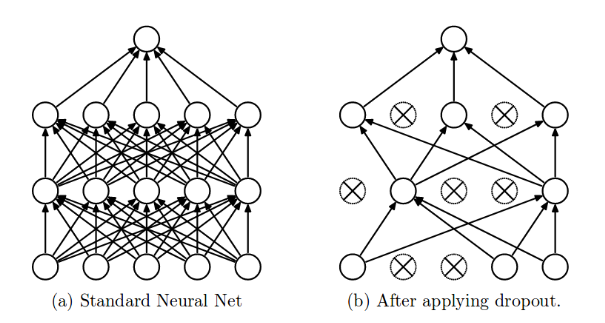
\includegraphics[width=0.7\textwidth]{figures/dropout.png}
        \caption{Dropout regularization}
        \label{fig:dropout}
    \end{figure}

\end{enumerate}

\section{Optimization methods: Gradient Descent}

The process of training a neural network involves solving an optimization problem
to minimize the loss function. There are many optimization algorithms that can be
used to train a neural network. To study these algorithms, let us first define
some basic concepts.\\

Let us consider a function $f: \mathbb{R}^n \rightarrow \mathbb{R}$ convex and
differentiable. A convex function has these properties:

\begin{enumerate}
    \item The domain of $f$ is a convex set, i.e., for any $x, y \in \text{dom}(f)$:
    $$\lambda x + (1 - \lambda) y \in \text{dom}(f)$$

    \item For any $x, y \in \text{dom}(f)$ and $\lambda \in [0, 1]$:
    $$f(\lambda x + (1 - \lambda) y) \leq \lambda f(x) + (1 - \lambda) f(y)$$
\end{enumerate}

Now, let us propose the following optimization problem:

\begin{equation}
    \min_{x \in \mathbb{R}^n} f(x)
\end{equation}

An idea to solve this problem is to propose an iterative algorithm such that, starting from
an initial point $x^{(0)}$, we update the point $x^{(k)}$ to $x^{(k+1)}$ in such a way that:

$$x^{(k+1)} = \min_{x \in \R^n} \tilde{f}_k(x)$$
    
where $\tilde{f}_k$ is a function that approximates $f$ at the point $x^{(k)}$. Some ways to
approximate $f$ are:

\begin{enumerate}
    \item \textbf{Linear approximation}
    
    A linear approximation of $f$ at the point $x^{(k)}$ is given by:

    $$\tilde{f}_k(x) = c_k + b_k^T (x - x^{(k)})$$

    where $c_k$ is a scalar and $b_k$ is a vector. Right away, we notice that this problem
    is unbounded, and we need to add some constraints to make it feasible.\\

    \item \textbf{Quadratic approximation}
    
    A quadratic approximation of $f$ at the point $x^{(k)}$ is given by:

    $$\tilde{f}_k(x) = c_k + b_k^T (x - x^{(k)}) + \frac{1}{2} (x - x^{(k)})^T A_k (x - x^{(k)})$$

    where $A_k$ is a matrix. Let us use this form of approximation, and set some conditions:

    \begin{enumerate}
        \item $f(x^{(k)}) = \tilde{f}_k(x^{(k)})$
        \item $\nabla \tilde{f}_k(x^{(k)}) = \nabla f(x^{(k)})$
    \end{enumerate}

    From the first condition, we have:
    $$c_k = f(x^{(k)})$$

    From the second condition, we have:
    $$b_k = \nabla f(x^{(k)})$$

    Then, let us set $A_k = \frac{1}{\eta} I$, where $\eta$ is a positive scalar. Then,
    we have:

    $$\tilde{f}_k(x) = f(x^{(k)}) + \nabla f(x^{(k)})^T (x - x^{(k)}) + \frac{1}{2 \eta} \| x - x^{(k)} \|^2$$

    Now, notice that, since the function $\tilde{f}_k$ is convex, we can minimize it by
    setting the gradient to zero. Then, we have:

    $$\nabla \tilde{f}_k(x) = \nabla f(x^{(k)}) + \frac{1}{\eta} (x - x^{(k)}) = 0$$
    $$\Rightarrow x^{(k+1)} = x^{(k)} - \eta \nabla f(x^{(k)})$$

    This is the \textbf{gradient descent algorithm}, and we call $\eta$ the learning rate.\\
\end{enumerate}

\subsection{Gradient descent algorithm}

More formally, the gradient descent algorithm is defined as follows, for a function
$f: \R^n \rightarrow \R$:

\begin{algorithm}[H]
    \caption{Gradient descent algorithm}
    \begin{algorithmic}[1]
        \Require $x^{(0)}, \eta, \varepsilon, T$
        \For{$k = 0, 1, 2, \ldots, T$}
            \State $x^{(k+1)} = x^{(k)} - \eta \nabla f(x^{(k)})$
            \If{\textbf{STOP}$(\varepsilon)$}
                \State \textbf{break}
            \EndIf
        \EndFor
    \end{algorithmic}
\end{algorithm}

In this case, we can define the stopping criterion as:

\begin{equation}
    \textbf{STOP}(\varepsilon) = \left\{ \begin{array}{ll}
        \text{true} & \text{if } \| \nabla f(x^{(k)}) \| \leq \varepsilon\\
        \text{false} & \text{otherwise}
    \end{array} \right.
\end{equation}

Or:

\begin{equation}
    \textbf{STOP}(\varepsilon) = \left\{ \begin{array}{ll}
        \text{true} & \text{if } |f(x^{(k+1)}) - f(x^{(k)})| \leq \varepsilon\\
        \text{false} & \text{otherwise}
    \end{array} \right.
\end{equation}

Or:

\begin{equation}
    \textbf{STOP}(\varepsilon) = \left\{ \begin{array}{ll}
        \text{true} & \text{if } \| x^{(k+1)} - x^{(k)} \| \leq \varepsilon\\
        \text{false} & \text{otherwise}
    \end{array} \right.
\end{equation}

Now, to choose the learning rate $\eta$, we have many options. One of them is to
use a fixed learning rate. Another option is to use a learning rate that decreases
over time. This is called the learning rate schedule, and effectively, just decreases
the learning rate depending on the iteration. For example:

\begin{equation}
    \eta_k = \frac{\eta_0}{1 + k}
\end{equation}

where $\eta_0$ is the initial learning rate. Another option is to use the \textbf{Backtracking
line search}, which is an algorithm that finds an effective learning rate at each iteration. It
works as follows:

\begin{algorithm}[H]
    \caption{Backtracking line search}
    \begin{algorithmic}[1]
        \Require $x^{(k)}, \eta_0, \alpha, \beta$
        \State $\eta = \eta_0$
        \While{$f(x^{(k)} - \eta \nabla f(x^{(k)})) > f(x^{(k)}) - \alpha \eta \| \nabla f(x^{(k)}) \|^2$}
            \State $\eta = \beta \eta$
        \EndWhile
    \end{algorithmic}
\end{algorithm}

We usually set $\alpha = 0.5$ and $\beta = 0.5$.\\

Another way of setting the learning rate is to use the \textbf{Exact line search}, which
is an algorithm that finds the optimal learning rate at each iteration. It works by solving
the following optimization problem at each iteration:

\begin{equation}
    \eta^{(k)} = \argmin_{\eta > 0} f(x^{(k)} - \eta \nabla f(x^{(k)}))
\end{equation}

This is a one-dimensional optimization problem that can be solved using standard optimization,
but it can be computationally expensive, as it may not have a closed-form solution. In practice,
the exact line search is rarely used.

\subsubsection{Wolfe conditions}

In general, a good learning rate is one that satisfies the \textbf{Wolfe conditions}. These are a 
set of conditions that ensure that the learning rate is not too large or too small. The Wolfe
conditions are defined as follows:\\

For $0 < c_1 < c_2 < 1$, and a descent direction $d$, the Wolfe conditions are:

\begin{enumerate}
    \item \textbf{Sufficient decrease condition:}
    $$f(x + \eta d) \leq f(x) + c_1 \eta \nabla f(x)^T d$$

    This condition ensures that the learning rate is not too large, i.e., that the function value
    decreases sufficiently at each iteration.

    \item \textbf{Curvature condition:}
    $$\nabla f(x + \eta d)^T d \geq c_2 \nabla f(x)^T d$$

    This condition ensures that the learning rate is not too small, i.e., that the gradient of the
    function is not too flat at each iteration.
\end{enumerate}

The Wolfe conditions are a good way to choose the learning rate, as they ensure that the learning
rate is not too large or too small. In practice, the Wolfe conditions are often used in conjunction
with the backtracking line search to find an effective learning rate at each iteration.

\subsection{Convergence of the gradient descent algorithm}

Let us state the following theorem:

\begin{theorem}
    Let $f: \R^n \rightarrow \R$ be a convex function that is differentiable and has a Lipschitz
    continuous gradient with constant $L$. Let $\{ x^{(k)} \}$ be the sequence generated by the
    gradient descent algorithm with learning rate $\eta \leq \frac{1}{L}$. Then, we have:

    \begin{equation}
        f(x^{(k)}) - f(x^*) \leq \frac{\| x^{(0)} - x^* \|^2}{2 \eta k}
    \end{equation}

    where $x^*$ is the optimal solution of the optimization problem.
\end{theorem}

\begin{proof}
    This proof is different from the one presented in the professor's lecture. Nonetheless, it
    is a valid proof. It is based on the following lemma:

    \begin{lemma}[Descent lemma]
        Let $f: \R^n \rightarrow \R$ be a differentiable function that has a Lipschitz
        continuous gradient with constant $L$. Then, for any $x, y \in \R^n$, we have:

        \begin{equation}
            f(y) \leq f(x) + \nabla f(x)^T (y - x) + \frac{L}{2} \| y - x \|^2
        \end{equation}
    \end{lemma}

    \begin{proof}
        Let us define the function $g(t) = f((1 - t) x + t y)$. Then, by the fundamental theorem
        of calculus, we have:
        
        \begin{align*}
            g(1) &= g(0) + \int_{0}^{1} g'(t) dt\\
            f(y)&= f(x) + \int_{0}^{1} \nabla f((1 - t) x + t y)^T (y - x) dt\\
                &= f(x) + \nabla f(x)^T (y - x) + \int_{0}^{1} (\nabla f((1 - t) x + t y) - \nabla f(x))^T (y - x) dt\\
        \end{align*}

        By the Cauchy-Schwarz inequality (more generally, the Hölder's inequality), we have:

        \begin{align*}
            (\nabla f((1 - t) x + t y) - \nabla f(x))^T(y - x) &\leq \| \nabla f((1 - t) x + t y) - \nabla f(x) \| \| y - x \|\\
        \end{align*}

        And then, by the Lipschitz continuity of the gradient, we have:

        \begin{align*}
            \|\nabla f((1 - t) x + t y)^T - \nabla f(x)^T\| &\leq L \| (1 - t) x + t y - x \|\\
            &= L t \| y - x \|
        \end{align*}

        Then, we have:

        \begin{align*}
            f(y) &\leq f(x) + \nabla f(x)^T (y - x) + \int_{0}^{1} L t \| y - x \|^2 dt\\
            &= f(x) + \nabla f(x)^T (y - x) + \frac{L}{2} \| y - x \|^2
        \end{align*}

        This is the desired result.

    \end{proof}


    Observe that a direct consequence of the descent lemma is that the gradient descent algorithm
    is in fact a descent algorithm, i.e., it decreases the value of the function at each iteration.
    We can propose our second lemma:

    \begin{lemma}[Gradient descent lemma]
        Let $f: \R^n \rightarrow \R$ be a function that is differentiable and has a Lipschitz
        continuous gradient with constant $L$. Let $\{ x^{(k)} \}$ be the sequence generated by the
        gradient descent algorithm with learning rate $\eta \leq \frac{1}{L}$. Then, we have:

        \begin{equation}
            f(x^{(k+1)}) \leq f(x^{(k)}) - \frac{\eta}{2} \| \nabla f(x^{(k)}) \|^2
        \end{equation}
    \end{lemma}

    \begin{proof}
        By the descent lemma, we have:

        \begin{align*}
            f(x^{(k+1)}) &\leq f(x^{(k)}) + \nabla f(x^{(k)})^T (x^{(k+1)} - x^{(k)}) + \frac{L}{2} \| x^{(k+1)} - x^{(k)} \|^2\\
            &= f(x^{(k)}) - \eta \| \nabla f(x^{(k)}) \|^2 + \frac{L}{2} \| \eta \nabla f(x^{(k)}) \|^2\\
            &= f(x^{(k)}) - \left(1 - \frac{L \eta}{2} \right) \eta  \| \nabla f(x^{(k)}) \|^2
        \end{align*}

        Now notice that, since $\eta \leq \frac{1}{L}$, we have:

        $$1 - \frac{L \eta}{2} \geq \frac{1}{2}$$

        Then, we have:

        $$f(x^{(k+1)}) \leq f(x^{(k)}) - \frac{\eta}{2} \| \nabla f(x^{(k)}) \|^2$$

        This is the desired result.
    \end{proof}

    Now, let us prove the theorem. To do so, let us define the following operator:

    $$V_{t} = \frac{\|x^{(t)} - x^*\|^2}{2}$$

    Then, we have:

    \begin{align*}
        V_{t+1} &= \frac{1}{2} \|x^{(t+1)} - x^*\|^2  = \frac{1}{2} \|x^{(t)} - \eta \nabla f(x^{(t)}) - x^*\|^2\\
                &= \frac{1}{2} \left[ \|x^{(t)} - x^*\|^2  + \eta^2 \| \nabla f(x^{(t)}) \|^2 - 2 \eta \nabla f(x^{(t)})^T (x^{(t)} - x^*) \right]\\
                &= V_t + \frac{\eta^2}{2} \| \nabla f(x^{(t)}) \|^2 - \eta \nabla f(x^{(t)})^T (x^{(t)} - x^*)\\
    \end{align*}

    Here, we use the fact that $f$ is convex, meaning that:

    $$f(x^*) \geq f(x^{(t)}) + \nabla f(x^{(t)})^T (x^* - x^{(t)})$$

    $$\Rightarrow \nabla f(x^{(t)})^T (x^{(t)} - x^*) \geq f(x^{(t)}) - f(x^*)$$

    Then, we have:

    \begin{align*}
        V_{t+1} &\leq V_t + \frac{\eta^2}{2} \| \nabla f(x^{(t)}) \|^2 - \eta (f(x^{(t)}) - f(x^*))
    \end{align*}

    Now, notice that, by the gradient descent lemma, we have:

    $$\frac{\eta}{2} \| \nabla f(x^{(t)}) \|^2 \leq f(x^{(t)}) - f(x^(t + 1))$$

    Replace this in the previous equation, we have:

    \begin{align*}
        V_{t+1} &\leq V_t + \frac{\eta^2}{2} \| \nabla f(x^{(t)}) \|^2 - \eta (f(x^{(t)}) - f(x^*))\\
                &\leq V_t + \eta (f(x^{(t)}) - f(x^{(t+1)})) - \eta (f(x^{(t)}) - f(x^*))\\
                &= V_t - \eta (f(x^{(t+1)}) - f(x^*))\\
    \end{align*}

    We obtain that:

    $$f(x^{(t+1)}) - f(x^*) \leq \frac{1}{\eta} (V_t - V_{t+1})$$

    Now, using the fact that for each step, the value of the function decreases, we have:

    \begin{align*}
        T(f(x^{(T)}) - f(x^*)) &\leq \sum_{t=0}^{T-1} (f(x^{(t+1)}) - f(x^*))\\
                               &\leq \frac{1}{\eta} \sum_{t=0}^{T-1} (V_t - V_{t+1})\\
    \end{align*}

    Notice that the sum on the right-hand side telescopes, and we obtain:

    $$T(f(x^{(T)}) - f(x^*)) \leq \frac{1}{\eta} (V_0 - V_T) \leq \frac{1}{\eta} V_0$$

    Rearranging, we obtain:

    $$f(x^{(T)}) - f(x^*) \leq \frac{\| x^{(0)} - x^* \|^2}{2 \eta T}$$

    This is the desired result.

\end{proof}

\vspace{5em}

The result of the theorem can be generalized when used the backtracking line search. In this case,
we have:

\begin{equation}
    f(x^{(k)}) - f(x^*) \leq \frac{1}{2 \eta_{\min} k} \| x^{(0)} - x^* \|^2
\end{equation}

where $\eta_{\min} = \min \{1, \beta / L\}$.\\

With this result, we can calculate the number of iterations needed to reach a certain level of
accuracy. For example, if we want to reach an accuracy of $\varepsilon$, we have:

\begin{equation}
    k \geq \frac{1}{2 \eta \varepsilon} \| x^{(0)} - x^* \|^2 \in O\left(\frac{1}{\varepsilon}\right)
\end{equation}

This means that the gradient descent algorithm converges at a rate of $O(1/\varepsilon)$, called
\textbf{sub-linear convergence}. 


\subsection{Stochastic gradient descent (SGD)}

The gradient descent algorithm is a simple and effective optimization algorithm that can be used
to train a neural network. However, the gradient descent algorithm can be slow to converge when
the training data is large. This is because the gradient descent algorithm computes the gradient
of the loss function with respect to all the training data at each iteration. This can be
computationally expensive, especially when the training data is large.\\

To overcome this problem, we can use the stochastic gradient descent algorithm. The stochastic
gradient descent algorithm is a variant of the gradient descent algorithm that computes the
gradient of the loss function with respect to a random sample of the training data at each
iteration. This can be much faster than computing the gradient with respect to all the training
data.\\

The stochastic gradient descent algorithm works as follows:

\begin{algorithm}[H]
    \caption{Stochastic gradient descent algorithm}
    \begin{algorithmic}[1]
        \Require $x^{(0)}, \eta, \varepsilon, T$
        \For{$k = 0, 1, 2, \ldots, T$}
            \State Sample a random batch of training data $\{ x_i, y_i \}_{i=1}^m$
            \State Compute the gradient of the loss function with respect to the batch
            \State Update the weights of the model using the gradient
            \If{\textbf{STOP}$(\varepsilon)$}
                \State \textbf{break}
            \EndIf
        \EndFor
    \end{algorithmic}
\end{algorithm}

The sample can be chosen using one of the following strategies:

\begin{enumerate}
    \item Random sampling \textbf{with replacement}:\\
    In this strategy, in every iteration, we sample $m$ samples from the training data with replacement,
    i.e., we can sample the same sample more than once. To implement that, for each iteration, we have
    to choose a new set of indices to sample.

    \item Random sampling \textbf{without replacement}:\\
    In this strategy, in every iteration, we sample $m$ samples from the training data without replacement,
    i.e., we can sample the same sample only once. To implement that, we just shuffle the training data
    once and then go through the shuffled data in batches of size $m$.
\end{enumerate}

In practice, the second strategy is more common, as it can be more efficient. For every epoch of
training, we shuffle the training data and then go through the shuffled data in batches of size $m$.\\

Also, note that SGD is originally formulated by taking just one sample at a time, i.e., $m = 1$.
When $m > 1$, we call it \textbf{mini-batch stochastic gradient descent}.

\subsection{Convergence of SGD}

To study the convergence of the SGD algorithm, we will make some assumptions:

\begin{enumerate}
    \item $|u^T H_J u| \leq L \|u\|^2, ,\; L > 0$, where $H_J$ is the Hessian of the loss function.
    
    \item The loss function $J$ is $\mu$-strongly convex, i.e., for all $x, y \in \R^n$:
    $$J(y) \geq J(x) + \nabla J(x)^T (y - x) + \frac{\mu}{2} \|y - x\|^2$$

    \item $\|\nabla J_i(x)\| < C$ for all $i$ and $x$, where $C$ is a constant. Note 
    that $J(x) = \frac{1}{m} \sum_{i=1}^m J_i(x)$ for $m$ the number of samples.

    \item $\E[\nabla J_i(x)] = \nabla J(x)$. This means that $\nabla J_i(x)$ is an unbiased
    estimator of the gradient of the loss function.

    \item $0 < \eta \leq \frac{1}{2\mu}$, where $\eta$ is the learning rate.
\end{enumerate}

From the first assumption, we obtain that:

\begin{equation}
    J(y) \leq J(x) + \nabla J(x)^T (y - x) + \frac{L}{2} \|y - x\|^2
\end{equation}

And from the second assumption, we have:

\begin{equation}
    J(x^*) \geq J(x) - \frac{1}{2 \mu} \| \nabla J(x) \|^2
\end{equation}

Now, we would like to find an upper bound for these two differences:

\begin{itemize}
    \item $J(w^{k}) - J(w^*)$
    \item $\|w^{(k)} - w^*\|^2$
\end{itemize}

Lets us start with the first one. By using the SGD step and the first assumption, we have:

\begin{align*}
    J(w^{(k+1)}) &\leq J(w^{(k)}) + \nabla J(w^(k))^T (w^{(k+1)} - w^{(k)}) + \frac{L}{2} \|w^{(k+1)} - w^{(k)}\|^2\\
                 &= J(w^{(k)}) - \eta \nabla J(w^{(k)})^T \nabla J_i(w^{(k)}) + \frac{L \eta^2}{2} \| \nabla J_i(w^{(k)}) \|^2\\
                 &\leq J(w^{(k)}) - \eta \nabla J(w^{(k)})^T \nabla J_i(w^{(k)}) + \frac{L \eta^2}{2} C^2
\end{align*}

Now, bt subtracting $J(w^*)$ from both sides, we have:

\begin{align*}
    J(w^{(k+1)}) - J(w^*) &\leq J(w^{(k)}) - J(w^*) - \eta \nabla J(w^{(k)})^T \nabla J_i(w^{(k)}) + \frac{L \eta^2}{2} C^2\\
\end{align*}

Now, we can take the expectation of both sides:

\begin{align*}
    \E[J(w^{(k+1)}) - J(w^*)] &\leq J(w^{(k)}) - J(w^*) - \eta \nabla J(w^{(k)})^T \E[\nabla J_i(w^{(k)})] + \frac{L \eta^2}{2} C^2\\
                              &= J(w^{(k)}) - J(w^*) - \eta \nabla J(w^{(k)})^T \nabla J(w^{(k)}) + \frac{L \eta^2}{2} C^2\\
                              &= J(w^{(k)}) - J(w^*) - \eta \| \nabla J(w^{(k)}) \|^2 + \frac{L \eta^2}{2} C^2
\end{align*}

Now, we can use the equation (3.37) to obtain:

$$- \| \nabla J(w^{(k)}) \|^2 \leq - 2 \mu (J(w^{(k)}) - J(w^*))$$

Then, we have:

\begin{align*}
    \E[J(w^{(k+1)}) - J(w^*)] &\leq J(w^{(k)}) - J(w^*) - 2 \mu \eta (J(w^{(k)}) - J(w^*)) + \frac{L \eta^2}{2} C^2\\
                              &= (1 - 2 \mu \eta) (J(w^{(k)}) - J(w^*)) + \frac{L \eta^2}{2} C^2
\end{align*}

Now, notice that we have the following inequality:

$$\E[J(w^{(k+1)}) - J(w^*)] \leq (1 - 2 \mu \eta) \E[J(w^{(k)}) - J(w^*)] + \frac{L \eta^2}{2} C^2$$

If we reapply the expected value to the equation, the left-hand side will remain the same (as
the expectation is a constant value), and we will have:

$$\E[J(w^{(k+1)}) - J(w^*)] \leq (1 - 2 \mu \eta) \E[J(w^{(k)}) - J(w^*)] + \frac{L \eta^2}{2} C^2$$

This is a recursive equation. We get as solution:

$$\E[J(w^{(k)}) - J(w^*)] \leq (1 - 2 \mu \eta)^k (J(w^{(0)}) - J(w^*)) + \frac{L \eta^2}{2} C^2 \sum_{i=0}^{k-1} (1 - 2 \mu \eta)^i$$

Now, we can use the geometric series formula to obtain:

$$\sum_{i=0}^{k-1} (1 - 2 \mu \eta)^i = \frac{1 - (1 - 2 \mu \eta)^k}{2 \mu \eta}$$

And notice that, since $0 < \eta \leq \frac{1}{2 \mu}$, we have:

$$0 < 1 - 2 \mu \eta < 1$$

So we have:

$$ \frac{1 - (1 - 2 \mu \eta)^k}{2 \mu \eta} \leq \frac{1}{2 \mu \eta}$$

Using this result, we have:

\begin{equation}
    \E[J(w^{(k)}) - J(w^*)] \leq (1 - 2 \mu \eta)^k (J(w^{(0)}) - J(w^*)) + \frac{L \eta}{4 \mu} C^2
\end{equation}

Notice that the term $(1 - 2 \mu \eta)^k$ is a decreasing function of $k$. This means that the
expected value of the loss function decreases with the number of iterations, with
exception of the term $\frac{L \eta}{4 \mu} C^2$. This term is a constant value that depends on
the learning rate $\eta$ and the constants $L$, $\mu$ and $C$. This is why we need to choose the
learning rate carefully, as it can affect the convergence of the algorithm.\\

Similarly, we can obtain an upper bound for the expected value of the second term, 
$\|w^{(k)} - w^*\|^2$:

\begin{equation}
    \E[\|w^{(k)} - w^*\|^2] \leq (1 - 2 \mu \eta)^k \|w^{(0)} - w^*\|^2 + \frac{\eta}{2\mu} C^2
\end{equation}

This means that the expected value of the distance between the weights and the optimal solution
also decreases with the number of iterations, with exception of the term $\frac{\eta}{2\mu} C^2$.\\

This result shows that the SGD algorithm is expected to converge to some vicinity with radius
$\frac{\eta}{2\mu} C^2$ of the optimal solution. This is a good result, as it shows that the
SGD algorithm is able to find a good solution to the optimization problem.\\

However, notice that these results have strong assumptions, that in practice are not always
satisfied. For example, the assumption that the loss function is strongly convex is not always
true. In practice, the loss function is often non-convex, which can make the optimization problem
more difficult. 


\section{Improving the SGD: Momentum and Adaptive learning rates}

There are many techniques that can be used to improve the performance of the SGD algorithm.
Two of the most popular techniques are \textbf{momentum} and \textbf{adaptive learning rates}.
These techniques can help to speed up the convergence of the SGD algorithm and improve the
performance of the model.\\

In this section, we will discuss the following algorithms:

\begin{itemize}
    \item SGD with momentum
    \item Nesterov accelerated gradient (NAG)
    \item AdaGrad
    \item AdaDelta + RMSProp
    \item Adam
\end{itemize}

\subsection{SGD with momentum}

The SGD with momentum algorithm is a variant of the SGD algorithm that uses a momentum term to
accelerate the convergence of the algorithm. The momentum term is a moving average of the
gradients of the loss function. This can help to smooth out the updates to the weights and
improve the performance of the model.\\

It's step is given by:

\begin{equation}
    \begin{aligned}
        v^{(k+1)} &= \gamma v^{(k)} + \eta \nabla J(w^{(k)}) \\
        w^{(k+1)} &= w^{(k)} - v^{(k+1)}
    \end{aligned}
\end{equation}

Note that $v^{(k)}$ represents the momentum term, and $\gamma$ is the momentum parameter. The
momentum parameter is a hyperparameter that controls the influence of the momentum term on the
updates to the weights.\\

The momentum term allows us to take into account the previous gradients when updating the weights.
In some way, we are considering the velocity of the descent, and not only the gradient at the
current point. This helps us to avoid local minima and saddle points, in which the gradient is
close to zero.

\subsection{Nesterov accelerated gradient (NAG)}

The Nesterov accelerated gradient (NAG) algorithm is a variant of the SGD with momentum algorithm
that uses a different update rule for the weights. The NAG algorithm uses the gradient of the
loss function at the point $w^{(k)} - \gamma v^{(k)}$ to update the weights. The step
of the NAG algorithm is given by:

\begin{equation}
    \begin{aligned}
        v^{(k+1)} &= \gamma v^{(k)} + \eta \nabla J(w^{(k)} - \gamma v^{(k)}) \\
        w^{(k+1)} &= w^{(k)} - v^{(k+1)}
    \end{aligned}
\end{equation}

In this case, the expression $\nabla J(w^{(k)} - \gamma v^{(k)})$ is an approximation of the
gradient of the loss function at the point $w^{(k+1)}$. The term $w^{(k)} - \gamma v^{(k)}$ is
known as a \textbf{predictor corrector} step, as we are in some way "looking ahead" to the value
of the gradient at the possible next point. Then we use this to calculate the real update to the
weights. This can help to improve the performance of the algorithm and speed up the convergence.

\subsection{AdaGrad}

The AdaGrad algorithm is a variant of the SGD algorithm that uses an adaptive learning rate to
update the weights. The AdaGrad algorithm uses a different learning rate for each weight, based
on the history of the gradients of the loss function. The step of the AdaGrad algorithm is given
by:

\begin{equation}
    \begin{aligned}
        G^{(k)} &= G^{(k-1)} + (\nabla J(w^{(k)}))^2 \\
        w^{(k+1)} &= w^{(k)} - \eta_0 (G^{(k)} + \varepsilon \cdot \1)^{-1/2} \odot \nabla J(w^{(k)})
    \end{aligned}
\end{equation}

Here, $G^{(k)}$ contains the sum of the squares of the gradients of the loss function up to the
$k$-th iteration. The term $\varepsilon$ is a small constant that is added to the denominator to
avoid division by zero. The term $\1$ is a vector of ones with the same size as the weights. The
term $(G^{(k)} + \varepsilon \cdot \1)^{-1/2}$ is the element-wise inverse square root of the
sum of the squares of the gradients. This term is used to scale the gradients of the loss function
before updating the weights.\\

The AdaGrad algorithm adapts the learning rate for each weight based on the history of the gradients
of the loss function. This can help to improve the performance of the algorithm and speed up the
convergence.\\

However, the AdaGrad algorithm has some limitations. As the sum of the squares of the gradients increases, the learning rate decreases. This
can cause the learning rate to become very small, which can slow down the convergence of the
algorithm. To overcome this problem, we can use the AdaDelta algorithm.

\subsection{AdaDelta (and RMSProp)}

This algorithm is a variant of the AdaGrad algorithm that uses an adaptive learning rate to update
the weights. But in this case, instead of using the sum of the squares of the gradients up to the
$k$-th iteration, we use a moving average of the squares of the gradients, i.e., we take the average 
of the squares of the gradients on the last $n$ iterations.\\

Since keeping track of the last $n$ gradients can be computationally expensive, we can use an
exponential moving average to approximate the moving average. The step of the AdaDelta algorithm
is given by:

\begin{equation}
    \begin{aligned}
        E[g^2]^{(k)} &= \rho E[g^2]^{(k-1)} + (1 - \rho) (\nabla J(w^{(k)}))^2 \\
        \Delta w^{(k+1)} &= - \eta_0 (E[g^2]^{(k)} + \varepsilon \cdot \1)^{-1/2} \odot \nabla J(w^{(k)}) \\
        w^{(k+1)} &= w^{(k)} + \Delta w^{(k+1)}
    \end{aligned}
\end{equation}

where $E[g^2]^{(k)}$ is the notation for the moving average of the squares of the gradients up to
the $k$-th iteration. The term $\rho$ is the decay rate of the moving average, that controls the
influence of the previous gradients on the moving average. The term $\varepsilon$ is a small constant
that is added to the denominator to avoid division by zero.\\

The term $\sqrt{E[g^2]^{(k+1)} + \varepsilon}$ is the element-wise square root of the moving average
of the squares of the gradients. It is called the \textbf{root mean square} (RMS) of the gradients. This
is why the AdaDelta algorithm is also known as the RMSProp algorithm, as we are using the RMS of the
gradients to update the weights.\\

In other words, if we define:

\begin{equation}
    RMS[g]^{(k)} = \sqrt{E[g^2]^{(k)} + \varepsilon \cdot \1}
\end{equation}

Then, the step of the AdaDelta algorithm can be written as:

\begin{equation}
    \begin{aligned}
        E[g^2]^{(k)} &= \rho E[g^2]^{(k-1)} + (1 - \rho) (\nabla J(w^{(k)}))^2 \\
        \Delta w^{(k)} &= - \frac{\eta_0}{RMS[g]^{(k)}} \odot \nabla J(w^{(k)})\\
        w^{(k+1)} &= w^{(k)} + \Delta w^{(k)}
    \end{aligned}
\end{equation}

The hyperparameter $\rho$ is usually set to a value close to 1, e.g., $\rho = 0.9$. \\

The algorithm also uses an unit corrector factor. It is based on the fact that the update term $\Delta w^{(k)}$
is not proportional to the units of the weights. To correct this, we use the RMS of the update term
$\Delta w^{(k)}$ to scale the update term, instead of a fixed learning rate $\eta_0$:

\begin{equation}
    \Delta w^{(k)} = - \frac{RMS[\Delta w]^{(k-1)}}{RMS[g]^{(k)}} \odot \nabla J(w^{(k)})
\end{equation}

So, the AdaDelta algorithm can be written as:

\begin{equation}
    \begin{aligned}
        E[g^2]^{(k)} &= \rho E[g^2]^{(k-1)} + (1 - \rho) (\nabla J(w^{(k)}))^2 \\
        \Delta w^{(k)} &= - \frac{RMS[\Delta w]^{(k-1)}}{RMS[g]^{(k)}} \odot \nabla J(w^{(k)})\\
        E[\Delta w^2]^{(k)} &= \rho E[\Delta w^2]^{(k-1)} + (1 - \rho) (\Delta w^{(k)})^2\\
        w^{(k+1)} &= w^{(k)} + \Delta w^{(k)}\\
    \end{aligned}
\end{equation}

The idea of using the RMS of the gradients to update the weights is that it can help to avoid the
problem of the learning rate becoming very small, as in the AdaGrad algorithm. This allows the model
to adapt to the changing conditions of the optimization problem and keep learning even when the
gradients are small.

\subsection{Adam}

Adam is a very famous optimization algorithm that combines the ideas of the SGD with momentum and
the AdaDelta algorithm. The Adam algorithm uses a moving average of the gradients of the loss function
and the moving average of the squares of the gradients to update the weights. The step of the Adam
algorithm is given by:

\begin{equation}
    \begin{aligned}
        m^{(k)} &= \beta_1 m^{(k-1)} + (1 - \beta_1) \nabla J(w^{(k)}) \\
        v^{(k)} &= \beta_2 v^{(k-1)} + (1 - \beta_2) (\nabla J(w^{(k)}))^2 \\
        \hat{m}^{(k)} &= \frac{m^{(k)}}{1 - \beta_1^k} \\
        \hat{v}^{(k)} &= \frac{v^{(k)}}{1 - \beta_2^k} \\
        w^{(k+1)} &= w^{(k)} -  \frac{\eta_0}{\sqrt{\hat{v}^{(k)} + \varepsilon}} \odot \hat{m}^{(k)}
    \end{aligned}
\end{equation}

Here, $m^{(k)}$ is the moving average of the gradients of the loss function, $v^{(k)}$ is the moving
average of the squares of the gradients, $\beta_1$ and $\beta_2$ are the decay rates of the moving
averages, and $\varepsilon$ is a small constant that is added to the denominator to avoid division by
zero. The terms $\hat{m}^{(k)}$ and $\hat{v}^{(k)}$ are the bias-corrected moving averages, which are
used to correct the bias of the moving averages.\\

The Adam algorithm uses the moving average of the gradients to update the weights, and the moving
average of the squares of the gradients to scale the updates. This can help to improve the performance
of the algorithm and speed up the convergence. The hyperparameters $\beta_1$ and $\beta_2$ control the
influence of the moving averages on the updates to the weights. They are usually set to values close to
1, e.g., $\beta_1 = 0.9$ and $\beta_2 = 0.999$.\\

The Adam algorithm is a very powerful optimization algorithm that is widely used in practice. It can
help to improve the performance of the model and speed up the convergence of the algorithm. It is
recommended to use the Adam algorithm when training a neural network, as it can help to achieve better
results in less time.

\section{2nd order optimization methods: Newton's method and BFGS}

The gradient descent algorithm (and its variants) is a first-order optimization algorithm, as it
uses the first derivative of the loss function to update the weights. However, there are also
second-order optimization algorithms that use the second derivative of the loss function to update
the weights. These algorithms can converge faster than first-order optimization algorithms, as they
take into account the curvature of the loss function.\\

In this section, we will discuss two second-order optimization algorithms: Newton's method and the
Broyden-Fletcher-Goldfarb-Shanno (BFGS) algorithm.

\subsection{Newton's method}

The Newton's method is derived from a quadratic approximation of the loss function. The idea is to
approximate the loss function with a quadratic function and then find the minimum of the quadratic
function. Let us consider the following quadratic approximation of the loss function $J$ at the point
$w^{(k)}$:

\begin{equation}
    J(w) \approx \tilde{J}(w) = J(w^{(k)}) + \nabla J(w^{(k)})^T (w - w^{(k)}) + \frac{1}{2} (w - w^{(k)})^T H_J(w^{(k)}) (w - w^{(k)})
\end{equation}

Here, $H_J(w^{(k)})$ is the Hessian of the loss function at the point $w^{(k)}$. Now, we can find the
minimum of the quadratic function by setting the gradient of the quadratic function to zero:

$$\nabla \tilde{J}(w) = \nabla J(w^{(k)}) + H_J(w^{(k)}) (w - w^{(k)}) = 0$$

Solving this equation, we obtain:

\begin{equation}
    w = w^{(k)} - H_J(w^{(k)})^{-1} \nabla J(w^{(k)})
\end{equation}

This is the update rule of the Newton's method. In some way, this method uses the inverse of the
Hessian to adapt the direction of the gradient, according to the curvature of the loss function. 
Note that, in practice, we do not compute the inverse of the Hessian, and instead, we solve the
linear system $H_J(w^{(k)}) \Delta w = - \nabla J(w^{(k)})$ to find the update $\Delta w$.\\

We can also add a learning rate to the update rule to control the step size of the update:

\begin{equation}
    w^{(k+1)} = w^{(k)} - \eta H_J(w^{(k)})^{-1} \nabla J(w^{(k)})
\end{equation}

Similar to what happens in the gradient descent algorithm, the learning rate $\eta$ can be a fixed
value or can be adapted during training, and should follow the Wolfe conditions.\\ 

The Newton's method is a very powerful optimization algorithm that can converge very fast. However,
it has some limitations. One of the main limitations of the Newton's method is that it requires the
computation of the inverse of the Hessian of the loss function, which can be computationally expensive,
especially when the number of parameters is large. In practice, the inverse of the Hessian is often 
approximated using Quasi-Newton methods, such as the BFGS algorithm.

\subsection{Secant condition}

The methods for approximating the Hessian are based on the secant condition. To illustrate this,
let us consider the case of minimizing a one-dimensional function, $f: \R \rightarrow \R$. At
the $k+1$-th iteration, let us state the quadratic approximation of the function at the point $x^{(k+1)}$:

$$\tilde{f}^{(k+1)}(x) = f(x^{(k+1)}) + f'(x^{(k+1)}) (x - x^{(k+1)}) + \frac{1}{2} h(x^{(k+1)}) (x - x^{(k+1)})^2$$

Where $h(x^{(k+1)})$ is the approximation of the second derivative of the function at the point $x^{(k+1)}$.
On this approximation, we we want to enforce the following condition:

$$\tilde{f}^{(k+1)'}(x^{(k+1)}) = f'(x^{(k)})$$

This will allow us to determine an expression for $h(x^{(k+1)})$. By solving this equation, we obtain:

$$h(x^{(k+1)}) = \frac{f'(x^{(k+1)}) - f'(x^{(k)})}{x^{(k+1)} - x^{(k)}}$$

By using this expression on the update rule of the Newton's method, we obtain:

\begin{equation}
    x^{(k+1)} = x^{(k)} - \frac{f'(x^{(k)})}{h(x^{(k)})} = x^{(k)} - \frac{(x^{(k+1)} - x^{(k)})}{f'(x^{(k+1)}) - f'(x^{(k)})} f'(x^{(k)})
\end{equation}

This is called the secant method, for 1D functions. For multi-dimensional functions, we have the
same idea, but now we have to consider the Hessian matrix. Let us again propose a quadratic
approximation of the function at the point $x^{(k+1)}$:

$$\tilde{f}^{(k+1)}(x) = f(x^{(k+1)}) + \nabla f(x^{(k+1)})^T (x - x^{(k+1)}) + \frac{1}{2} (x - x^{(k+1)})^T \tilde{H}_f(x^{(k+1)}) (x - x^{(k+1)})$$

Where $\tilde{H}_f(x^{(k+1)})$ is the approximation of the Hessian of the function at the point $x^{(k+1)}$.
By enforcing the following condition:

$$\nabla \tilde{f}^{(k+1)}(x^{(k+1)}) = \nabla f(x^{(k)})$$

We can determine that the approximation of the Hessian should obey the following expression:

\begin{equation}
    \tilde{H}_f(x^{(k+1)}) (x^{(k+1)} - x^{(k)}) = \nabla f(x^{(k+1)}) - \nabla f(x^{(k)})
\end{equation}

This is the secant condition for multi-dimensional functions. But notice now that in this
expression, the unknown is the Hessian matrix, and not the second derivative of the function.
As the Hessian is symmetric, this means that for a $n \times n$ matrix, we have $n(n+1)/2$ unknowns.
The equation propose a total of $n$ conditions (one for each dimension). This means that we still
need to impose a total of:

$$\frac{n(n+1)}{2} - n = \frac{n(n-1)}{2}$$

additional conditions to solve the system. By formulating the rest of the conditions, we can
determine the approximation of the Hessian matrix. This is the idea behind the BFGS algorithm.\\

Before deducing the BFGS algorithm, let us repropose the secant condition in a more general form:

\begin{equation}
    H_{k+1} s_{k} = y_{k}
\end{equation}

where:

$$ s_{k} = x^{(k+1)} - x^{(k)}, \quad y_{k} = \nabla f(x^{(k+1)}) - \nabla f(x^{(k)})$$

Also notice that we are reformulating the notation of the Hessian matrix, as $H_{k+1}$, to indicate
that on each iteration, we have a different approximation of the Hessian, that should fullfil the previous
secant condition.

\subsection{BFGS algorithm}

This algorithm is named after Broyden, Fletcher, Goldfarb, and Shanno, who proposed the algorithm in
the 1970s. The BFGS algorithm is a Quasi-Newton method that uses the secant condition to approximate
the Hessian of the loss function. The BFGS algorithm enforces also the following conditions:

\begin{itemize}
    \item $H_{k+1}$ is symmetric
    \item $H_{k+1}$ is positive definite
    \item $H_{k+1}$ is a good approximation of the previous Hessian matrix $H_k$
\end{itemize}

In other words, the BFGS algorithm proposes the following problem to solve:

\begin{align*}
    \min_{H_{k+1}} &\| H_{k+1} - H_k \|_F^2\\
    \text{s.t. } &H_{k+1} s_{k} = y_{k}\\
                 &H_{k+1} \text{ is symmetric}
\end{align*}

Where $\| \cdot \|_F$ is the Frobenius norm. Now, since what we really want is to find the inverse 
of the Hessian, we can define the matrix $B_{k+1} = H_{k+1}^{-1}$, and then solve the following problem:

\begin{align*}
    \min_{B_{k+1}} &\| B_{k+1} - B_k \|_F^2\\
    \text{s.t. } &B_{k+1} y_{k} = s_{k}\\
                 &B_{k+1} \text{ is symmetric}
\end{align*}

To solve this problem, the algorithm proposes the following update rule to the Hessian:

$$H_{k+1} = H_k + a u u^T + b v v^T$$

where $u, v$ are linear independent vectors and $a, b$ are scalars. This is called a rank-2 update
to the Hessian. By imposing the secant condition, we obtain:

\begin{equation*}
    u = y_k, \quad v = H_k s_k, \quad a = \frac{1}{y_k^T s_k}, \quad b = - \frac{1}{s_k^T H_k s_k}
\end{equation*}

So, the update rule to the Hessian is given by:

\begin{equation}
    H_{k+1} = H_k + \frac{y_k y_k^T}{y_k^T s_k} - \frac{H_k s_k s_k^T H_k}{s_k^T H_k s_k}
\end{equation}

But notice that we are interested in the inverse of the Hessian, not the Hessian itself. So, we can
compute $B_{k+1} = H_{k+1}^{-1}$ by using the \textbf{Sherman-Morrison formula}:

\begin{equation}
    (A + UCV)^{-1} = A^{-1} - A^{-1} U (C^{-1} + V A^{-1} U)^{-1} V A^{-1}
\end{equation}

We can use this formula by defining:

\begin{equation*}
    A = H_k, \quad U = \begin{bmatrix}
        H_k s_k & y_k
    \end{bmatrix}, \quad C =\begin{bmatrix}
        \frac{-1}{s_k^T H_k s_k} & 0\\
        0 & \frac{1}{y_k^T s_k}
    \end{bmatrix}, \quad V = \begin{bmatrix}
        H_k s_k\\
        y_k
    \end{bmatrix}
\end{equation*}
        
By using the Sherman-Morrison formula, we can obtain the update rule to the inverse of the Hessian:

\begin{equation}
    B_{k+1} = (I - \rho s_k y_k^T) B_k (I - \rho y_k s_k^T) + \rho s_k s_k^T
\end{equation}

where:

$$\rho = \frac{1}{y_k^T s_k}$$

This is the final update rule of the BFGS algorithm. But we still need to ensure that the matrix
$B_{k+1}$ is positive definite. Let us consider the generic vector $z$:

\begin{align*}
    z^T B_{k+1} z &= (z - \rho s_k^T z y_k)^T B_k (z - \rho s_k^T z y_k) + \rho (s_k^T z)^2
\end{align*}

Now, as long as $B_k$ is positive definite, the term $(z - \rho s_k^T z y_k)^T B_k (z - \rho s_k^T z y_k)$
is positive. The term $\rho (s_k^T z)^2$ is also positive, if and only if $\rho > 0$. This means
that the matrix $B_{k+1}$ is positive definite, as long as we start with a positive definite matrix
$B_0$ and $\rho > 0$.\\

The condition $\rho > 0$ (also formulated as $y_k^T s_k > 0$) is called the \textbf{curvature condition}.
This condition ensures that the update to the inverse of the Hessian is positive definite. For strongly
convex functions, this condition is always satisfied. For other functions, we need to impose this
condition in some way, for example, by finding a point $x_{k+1}$ that satisfies Wolfe conditions, which
entail that the curvature condition is satisfied, using line search.\\

To initialize the BFGS algorithm, we need to start with a positive definite matrix $B_0$. A common
choice is to start with the identity matrix, $B_0 = I$. This is a good choice, as the identity matrix
is always positive definite and obviously symmetric.

\subsubsection{Low memory BFGS (L-BFGS)}

The BFGS algorithm requires the storage of the Hessian matrix, which can be computationally expensive
when the number of parameters is large. To overcome this problem, the low memory BFGS (L-BFGS) algorithm
was proposed.\\

Instead of storing the complete Hessian, L-BFGS stores only a few vectors that represent the approximation 
implicitly. Due to its resulting linear memory requirement, the L-BFGS method is particularly well suited 
for optimization problems with many variables.\\

Instead of the inverse Hessian $B_k$, L-BFGS maintains a history of the past m updates of the 
position $x$ and gradient $\nabla f(x)$, where generally the history size m 
can be small (often $m < 10$). These updates are used to implicitly do operations requiring 
the $B_k$-vector product.

\subsection{Comparison between Newton's method and BFGS}

The Newton's method and the BFGS algorithm are both second-order optimization algorithms that use the
second derivative of the loss function to update the weights. However, the main difference between the
two algorithms is the time complexity of computing the update rule.\\

Let us assume a problem of $n$ dimensions. The Newton's method requires the computation of the inverse
of the Hessian matrix, which has a time complexity of $O(n^3)$. This means that the Newton's method is
computationally expensive when the number of parameters is large.\\

On the other hand, the BFGS algorithm uses an approximation of the Hessian matrix, which can be computed
as we saw before. The time complexity of these matrix-vector products is $O(n^2)$. This means that the
BFGS algorithm is more efficient than the Newton's method when the number of parameters is large.\\

In summary, the complexities are:

\begin{itemize}
    \item Newton's method: \textbf{$O(n^3)$}
    \item BFGS algorithm: \textbf{$O(n^2)$}
\end{itemize}

But on the other hand, the Newton's method is more accurate than the BFGS algorithm, as it uses the
exact Hessian matrix to update the weights. This means that the Newton's method can converge faster
than the BFGS algorithm. 


